\chapter{Diseño y análisis de casos de uso}
\label{analisisPreimplementacion}

En este capítulo, teniendo en cuenta el marco teórico explicado en el Estado del Arte (Cap. \ref{estadoArte}), se analizará qué funcionalidades básicas deben poder ser implementadas por las distintas tecnologías para definir el \textit{datapath} de los dispositivos \gls{iot}, con el fin de alcanzar los objetivos indicados en la Introducción (Cap. \ref{intro}). \\
\par
Para ello, se diseñarán distintos casos de uso para comparar así las características que ofrecen cada una distintas tecnologías en relación a su  integración de los dispositivos \gls{iot} en entornos \gls{sdn}. De forma adicional, se estudiará sobre que plataformas se desplegarán los casos de uso, asegurándose de que tienen todos los mecanismos necesarios para llevar a cabo las pruebas. 

\section{Funcionalidades básicas}

Como se ha podido ver en el capítulo del Estado del arte (Cap. \ref{estadoArte}), las tecnologías  P4 y \gls{xdp} tienen muchos puntos fuertes, y amabas permiten definir el \textit{datapath} del dispositivo en cuestión. Con \gls{xdp}, obtenemos un gran rendimiento ya que el procesamiento de los paquetes se realiza casi en la propia interfaz, no consume recursos de forma activa, ya que opera de forma reactiva a los paquetes que llegan a la interfaz. Por otro lado, se encuentra la tecnología P4, la cual propone hacer uso de un lenguaje agnóstico del hardware  para definir el datapath. Esto aporta mucha versatilidad a la hora de implementar nuevos protocolos, o nuevas especificaciones de estándares. \\

\par

Teniendo en cuenta estas premisas, se ha decidido plantear una serie de funcionalidades básicas que una hipotética mota \gls{iot} tendría que implementar. Estas funcionalidades se van a recoger en casos de uso, los cuales serán desarrollados con ambas tecnologías (P4 y \gls{xdp}) para poder concluir con cual de ellas es más sencillo/eficiente realizar la integración de los dispositivos \gls{iot} en entornos \gls{sdn}, tal y como se ha definido en el objetivo principal del presente \gls{tfg}. \\
\par

Los casos de uso que se plantean son los siguientes: 

\begin{itemize}
    \item   \textbf{Case01 - Drop}: En este caso de uso se quiere ver si es posible descartar paquetes.
    \item   \textbf{Case02 - Pass}: En este caso de uso se quiere comprobar si es posible dejar pasar los paquetes, sin afectarles el plano de datos programado con la tecnología.
    \item   \textbf{Case03 - Echo server}: Este caso de uso, aunque se desarrollará un servidor el cual contestará todos los \texttt{ECHO-Resquest} que le lleguen, lo que se quiere ver es la facilidad que tenemos con ambas tecnologías de filtrar/parsear paquetes en base a sus cabeceras.
    
    \item   \textbf{Case04 - Layer 3 forwarding}: Con este caso de uso se comprobará qué tan sencillo es reenviar paquetes desde una interfaz a otra del dispositivo. 
    
    \item   \textbf{Case05 - Broadcast}: Por último, con este caso de uso se quería abordar cómo se puede conseguir  la difusión (o broadcast) de un hipotético paquete, es decir, si es posible clonar paquetes con las tecnologías o, en su lugar, crearlos de cero. 
\end{itemize}

Una vez definidas las funcionalidades a desarrollar con ambas tecnologías, se debe decidir sobre qué elementos se van a probar. En el caso de \gls{xdp} es sencillo, ya que como se explicó en el Estado del arte, los programas \gls{xdp} pueden ser cargados en la mayoría de interfaces gestionadas por el Kernel de Linux. \\
\par

%%%%%%%%%%%%%%%%%%%%%%%
% figura XDP process
\begin{figure}[ht]
    \centering
    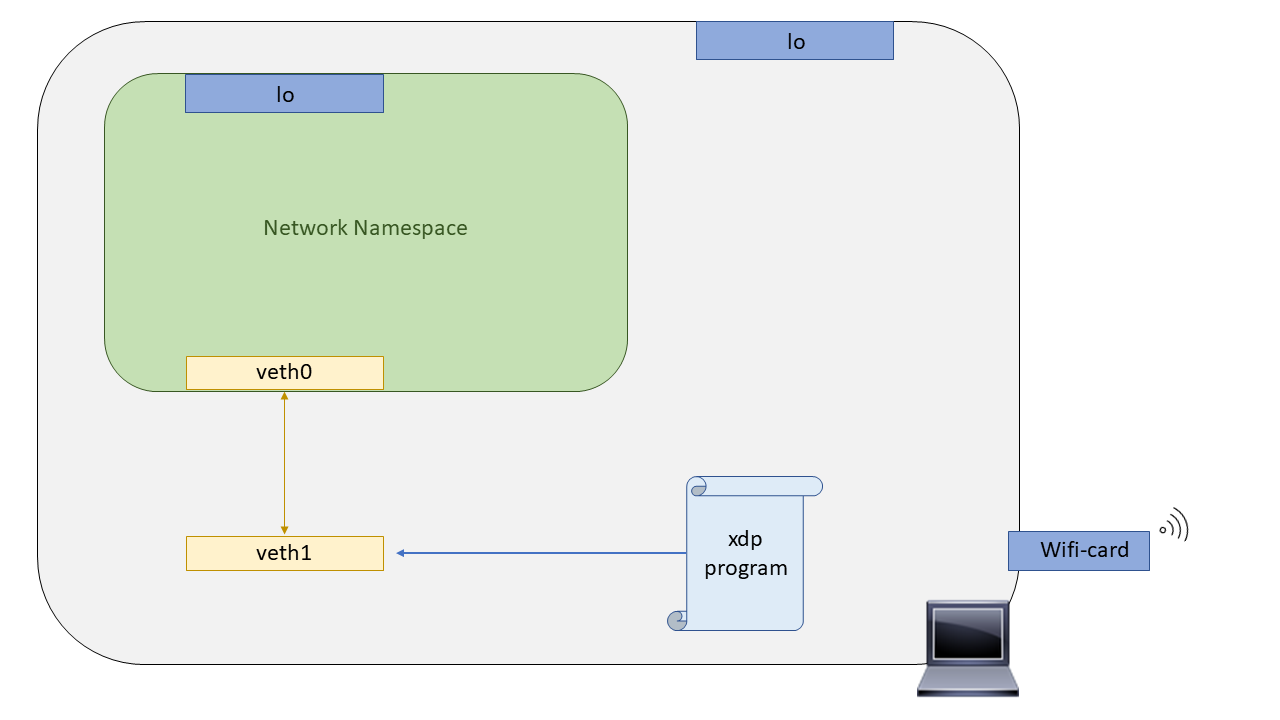
\includegraphics[width=14cm]{archivos/img/analisis/xdp_process.png}
    \caption{Ejemplo de carga de un programa XDP sobre una interfaz Ethernet virtual}
    \label{fig:xdp_process}
\end{figure}
%%%%%%%%%%%%%%%%%%%%%%%


En el caso de los programas P4 sí será necesario hacer uso de un elemento adicional para probar la funcionalidad desarrollada. Dicho elemento es el \gls{bmv2} \cite{p42018behavioral}, un soft-switch\footnote{ Switch virtual que se implementa a nivel de software.} desarrollado con la finalidad de probar código P4. Como se puede apreciar en la figura \ref{fig:p4_process}, el programa P4 una vez compilado se obtendrá un fichero JSON \cite{json} resultante que será el que le indique al \gls{bmv2} qué \textit{datapath} debe implementar.\\
\par

%%%%%%%%%%%%%%%%%%%%%%%
% figura P4 process
\begin{figure}[t]
    \centering
    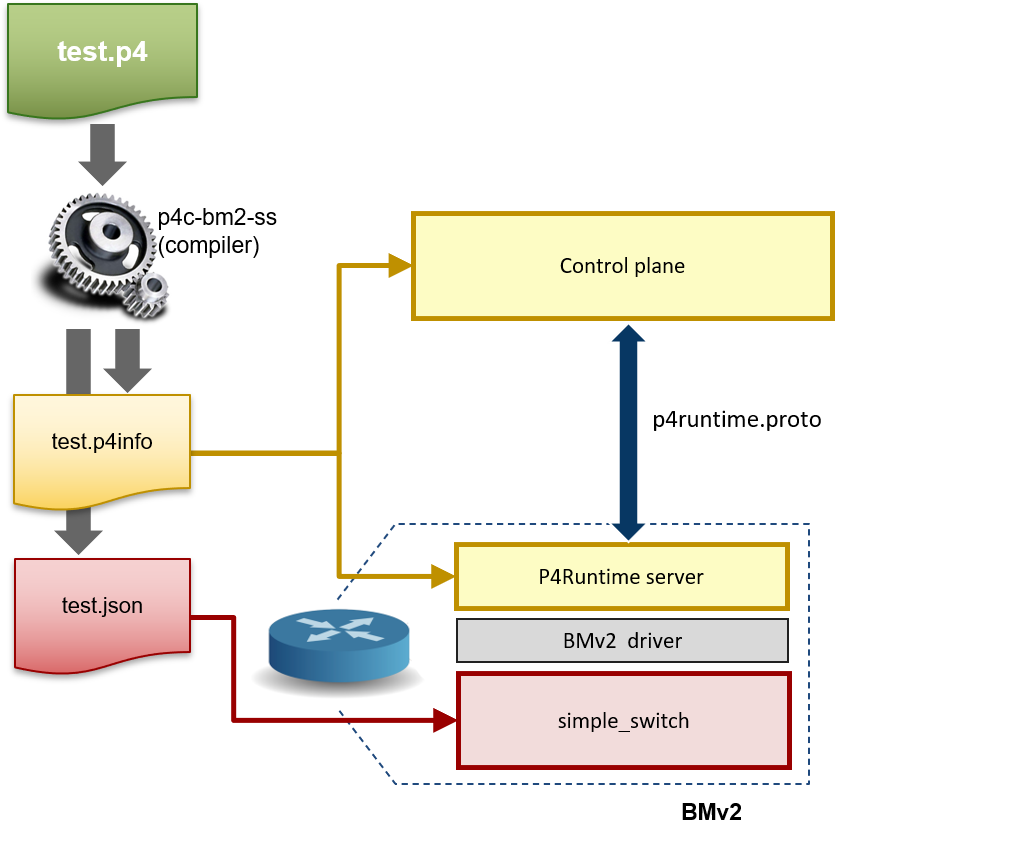
\includegraphics[width=11cm]{archivos/img/analisis/bmv2_process.png}
    \caption{Ejemplo de carga de un programa P4 sobre el BMV2}
    \label{fig:p4_process}
\end{figure}
%%%%%%%%%%%%%%%%%%%%%%%


Atendiendo a los modelos de integración de dispositivos \gls{iot} comentados en la Introducción \ref{sdn_iot_parcial} y \ref{sdn_iot_total}, se van a desarrollar casos de uso tanto en entornos  \textbf{cableados} como para entornos  \textbf{inalámbricos}. La motivación de esta decisión se basa en que, como se puede ver en la figura \ref{sdn_iot_parcial}, habrá dispositivos híbridos \gls{iot} mediadores, los cuales estarán parcialmente conectados al core \gls{sdn} de manera cableada, y de manera inalámbrica con el resto de dispositivos \gls{iot}. Por ello, se estima necesario comprobar el rendimiento de ambas tecnologías en ambos entornos , ya que ciertos dispositivos \gls{iot} en las integraciones parciales pueden ser favorecidos de igual manera. \\
\par

A continuación, se analizará sobre qué plataformas se llevará a cabo la evaluación de las funcionalidades básicas desarrolladas. Se elegirán plataformas para entornos cableados y para entornos  inalámbricos, intentando siempre hacer uso de un número mínimo de ellas para que así las evaluaciones sean lo más homogéneas posibles. 


\section{Plataformas de pruebas alámbricas}

Para evaluar los desarrollos de \gls{xdp} y P4 en entornos  cableados se hará uso del estándar \texttt{ieee8023} (Ethernet), aunque este estándar se diseñó en un principio para operar en redes de carácter local, con el paso de los años la tecnología Ethernet fue avanzando a la par que su popularidad, alcanzando tasas de transmisión de \textit{40 Gbit/s} con el estándar \texttt{ieee8023ba}\footnote{\url{http://www.ieee802.org/3/ba/}}. \\
\par

 Las evaluaciones de los programas \gls{xdp} serán realizadas sobre una plataforma Linux donde se generaran topologías de red conformadas por \textit{Network Namespaces}, para definir los nodos independientes de la red, y de \gls{veth}, para emular los enlaces entre distintos nodos. Todos los escenarios empleados serán suministrados en el repositorio del \gls{tfg} en forma de \textit{shellscript}, indicando al usuario cómo lanzar dicho escenario, y cómo hacer uso del mismo script para limpieza del escenario recreado. Se ha querido hacer uso de \textit{Network Namespaces} como plataforma para validar los desarrollos, ya que es la expresión más básica de emulación de redes en el Kernel de Linux. De esta forma, y debido a la complejidad que supone trabajar con programas \gls{xdp}, se buscaba que la plataforma donde se fueran a evaluar los casos de uso aportase la mínima incertidumbre posible sobre los resultados obtenidos. \\

\par

En cuanto a la plataforma elegida para evaluar los programas P4, se hará uso de Mininet. Como ya se comentó en el Estado del Arte (Cap. \ref{estadoArte}), Mininet es una herramienta para la emulación de topologías de red \gls{sdn}, de la cual nació Mininet-WiFi añadiendo soporte para redes inalámbricas. Se ha elegido Mininet, debido a que el equipo de \textit{p4lang} desarrolló una interfaz\footnote{\url{https://github.com/p4lang/tutorials/tree/master/utils/mininet}} del \gls{bmv2} con dicha herramienta, de esta forma es posible incorporar el soft-switch de referencia para probar código P4, como un tipo de nodo más en Mininet. 
 

\section{Plataformas de pruebas inalámbricas}


Para evaluar los desarrollos de \gls{xdp} y P4 en entornos  inalámbricos se hará uso del estándar \texttt{ieee80211} (WiFi). Se ha elegido dicho estándar cómo un primer paso, debido a que a día de hoy, existen más herramientas y desarrollos que para el estándar \texttt{ieee802154}. El estándar \texttt{ieee80211} es uno de los estándares de redes inalámbricas más populares del mundo recibiendo constantes actualizaciones por parte del \gls{ieee} para mejorar su rendimiento, o dar soporte a nuevas funcionalidades \cite{gast2005802}. Siendo este grupo de trabajo uno de los más activos dentro del proyecto de estandarización del \gls{ieee} de redes de area local (Fig. \ref{fig:ieee802}).  \\
\par

%%%%%%%%%%%%%%%%%%%%%%%
% figura familia 802
\begin{figure}[ht]
    \centering
    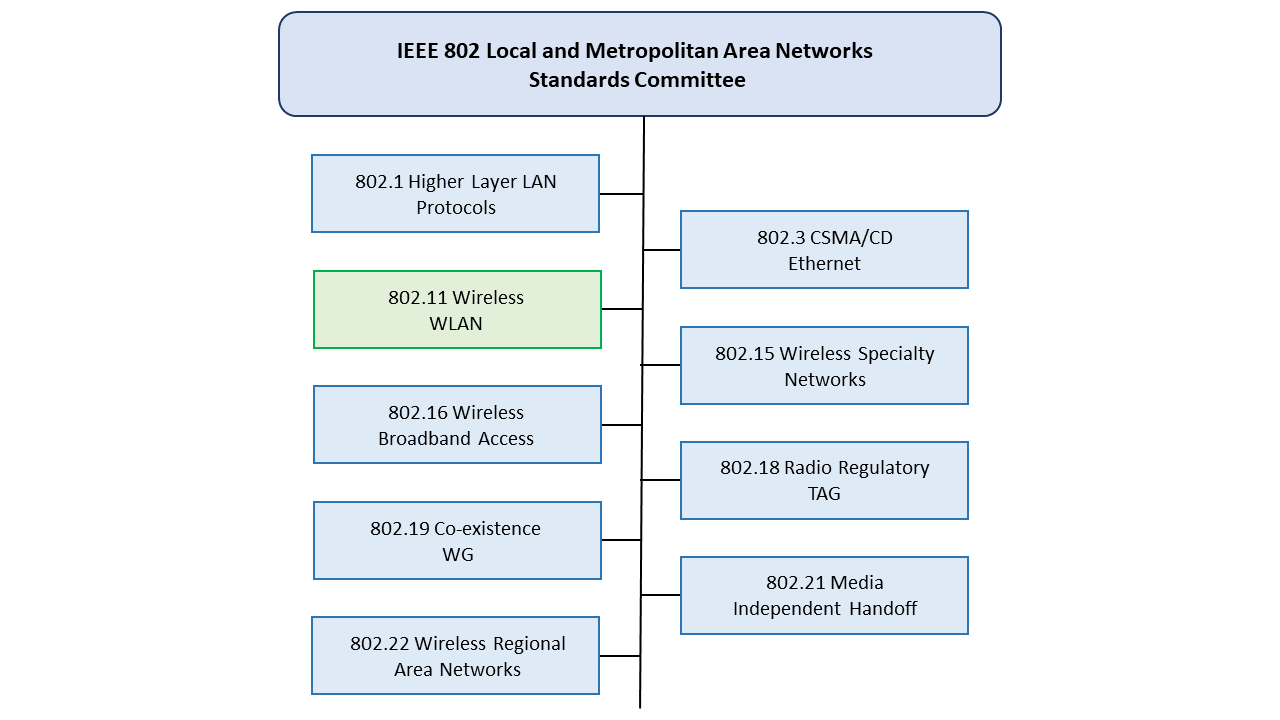
\includegraphics[width=15.5cm]{archivos/img/analisis/802_X_estandares_2.png}
    \caption{Grupos de trabajo IEEE 802}
    \label{fig:ieee802}
\end{figure}
%%%%%%%%%%%%%%%%%%%%%%%


La plataforma que se utilizará para la evaluación de los distintos casos de uso, tanto en \gls{xdp} como en P4, será la misma. Se hizo uso del emulador Mininet-WiFi en lugar del simulador Cooja para evaluar el funcionamiento de ambas tecnologías (XDP y P4) en entornos  inalámbricos. Esto se debe a que para probar ambas tecnologías se requiere de interfaces reales o emuladas donde poder evaluar el funcionamiento de los desarrollos. También se podría haber valorado hacer uso del emulador Mininet-IoT, pero como se menciono en la sección \ref{mininetIoT}, dicha herramienta se integró en Mininet-Wifi como un complemento más. Por lo que, eligiendo a Mininet-WiFi se tiene las nuevas funcionalidades de Mininet-IoT y además, cuenta con mayor madurez al llevar más años en la escena.\\


\par
En los desarrollos \gls{xdp}, el flujo de trabajo consistirá en a levantar la topología en Mininet-WiFi, a través de un script en Python que hará uso de la API de Mininet-WiFi para recrear el escenario, acto seguido se anclará el programa \gls{xdp} en las interfaces del nodo de la red que corresponda. En cuanto a los programas P4, se ha visto que la plataforma no contempla ningún tipo de nodo que de soporte al \gls{bmv2} por lo que será necesario desarrollar previamente una integración del \gls{bmv2} en Mininet-WiFi. Es importante comentar que durante el desarrollo de este \gls{tfg}, el desarrollador principal de Mininet-WiFi, profesor de de la IFBA, Ramon Fontes\footnote{\url{https://github.com/ramonfontes}} empezó de forma paralela una integración de P4 en Mininet-WiFi abriendo un \textit{Issue}\footnote{\url{https://github.com/intrig-unicamp/mininet-wifi/issues/295}} donde mencionaba cómo debía desarrollarse la integración. En dicho \textit{Issue}, se pudieron debatir los detalles de la implementación de los soft-switch P4 en Mininet-WiFi. Más adelante, en el capitulo de desarrollo se expondrá como se abordó la integración, explicando su pre-implementación y desarrollo. \\

\par

El desarrollo de esta integración será vital para el proyecto. Teniendo en cuenta que la evaluación de los programas P4 en entornos inalámbricos dependerá de si se es capaz de embeber el \gls{bmv2} en la arquitectura de Mininet-WiFi. Los pasos propuestos para llevar a cabo la integración son los siguientes:
\vspace{0.5cm}

\begin{itemize}
    \item  Estudio y análisis de la interfaz creada desde el equipo \textit{p4Lang}, del \gls{bmv2} con Mininet.
    \item Estudio del subsistema \textit{Wireless} de Linux, y análisis del funcionamiento interno de Mininet-WiFi. Este punto será de vital importancia, puesto que se debe tener un buena idea de cómo trabaja Mininet-WiFi a bajo nivel.
    \item   Desarrollo de la integración, se debe conseguir que el \gls{bmv2} gestione las interfaces que Mininet-WiFi cree en los nodos del tipo \gls{ap}. De forma adicional, se tendrá que conseguir que el \gls{bmv2} se capaz de correr dentro de una \textit{Network Namespace}. Esta condición fue impuesta por Ramon Fontes en el \textit{Issue} mencionado anteriormente. 
\end{itemize}

Esta condición debía conseguirse para evitar problemáticas de \textit{by-pass} en redes Ad-Hoc. No se podía tener corriendo en una misma \textit{Network Namespace} todos los \gls{bmv2}, ya que ciertos paquetes irían directamente al \gls{bmv2} final, sin seguir el camino dispuesto en la red emulada.\\

%%%%%%%%%%%%%%%%%%%%%%%%%%%%%%%%%%%%%%%%%%%%%%%%%%%%%%%%%%%%%%%%%%%%%%%%%%%%%%%%%%%%%%%%%%%%%%%%%

